\chapter{Furthering Usability and Efficiency of Massively Parallel Gaussian Process Regression as Applied to Multi-Beam Sonar Data}

\begin{centering} 

\vspace{.5in}

by 

\vspace{.5in}

Phillip M. Parisi\footnote{\label{note1} University of Rhode Island, Department of Ocean Engineering},
Chris Roman\textsuperscript{\ref{note1}}$^{,}$\footnote{\label{note2} University of Rhode Island, Graduate School of Oceanography},
Kristopher Krasnosky\footnote{\label{note3} University of South Florida, Center for Ocean Mapping and Innovative Technologies}


\vspace{1in}

\textit{In preparation for submission to the Journal of UNKNOWN}

\end{centering}

\newpage

\section{Introduction}

Multi-beam echo sounder (MBES) surveys repeatedly ping the seafloor using acoustic transducers to determine the water depth at points along the seafloor. These returns can contain upwards of one hundred datapoints and surveys that ping the seafloor for hours will result in millions of datapoints. Forming models of the seafloor from these data can be viewed as a regression problem. Regression, determining the relationship between a dependent variable and one or more independent variables, can be solved using Gaussian Process Regression (GPR) \cite{Rasmussen2006}. GPRs can be used to generate water depth predictions over a dense grid of points along the seafloor and calculate the associated uncertainties to provide a level of confidence in the predictions. Modern robotic algorithms that utilize probabilistic approaches benefit from GPR's uncertainty estimates in decision-making and estimation tasks. GPR has been applied to underwater terrain modeling \cite{barkby2012bathymetric-2}, terrain aided navigation (TAN) \cite{Hitchcox2020APC}, and simultaneous localization and mapping (SLAM) \cite{MA2018336, Krasnosky2022}. It is inefficient to compute GPR on large datasets; thus, utilizing a graphical processing unit (GPU) to reduce compute time has been explored \cite{FraneyGPU, Gramacy2013MP}. Krasnosky's Massively Parallel GPR (MP-GPR) was shown to improve the resolution of seafloor terrain models made from MBES data and generated an uncertainty model which other standard mapping methods (splines, gridded, polynomial, etc.) lack \cite{Krasnosky2022}. This work progresses Krasnosky's research by considering additional computational efficiencies and uncertainty from multi-beam sonar.



\subsection{Gaussian Process Regression}

 GPR is a supervised machine learning approach for determining input-output mappings from training data. The basic formulation of the problem uses empirical data points $D$ from a set of $N$ observations, known as \textit{training data}, consisting of inputs $\boldsymbol{x}$ (independent variables) and the corresponding targets $\boldsymbol{y}$ (dependent variable). Each observation $\boldsymbol{x}_i$ of $d$ dimensions maps to a scalar target $y_i$, which is a noisy realization of the underlying function of interest $f$.  
That is,
\begin{gather*}
    D = \{(\boldsymbol{x}_i,y_i)|i=1,\ldots,N\} \\
    \boldsymbol{x}\in\mathbb{R}^{N \times d}, \boldsymbol{y} \in\mathbb{R}^{N}, y_i = f(\boldsymbol{x}_i) + \epsilon,
\end{gather*}

where $\epsilon$ denotes error and bold symbols indicate matrix quantities. The error comes from sensor observation and is often assumed be normally distributed with zero mean, such that $\epsilon \sim \mathcal{N}(0,\sigma_n^{2})$. When applied to seafloor mapping, $\boldsymbol{x}_i = (\mathrm{northing}, \mathrm{easting})$ are the position variables and $y_i = \mathrm{depth}$ is the corresponding depth at that location. During the training portion of the problem, $D$ is used to learn the underlying function $f$.  During the inference step, $f$ is used to predict depths $\boldsymbol{y}^*$ over a new set of geographically dense inputs $\boldsymbol{x^*}$ to form a point cloud map.

An important component of any GPR model is the kernel which describes the relevant lengths scales and variance of the function being modeled. A commonly used kernel is the squared exponential (SE) kernel,
\begin{equation}
    k(\boldsymbol{x},\boldsymbol{x'}) = \sigma_f^2 exp(-\frac{|\boldsymbol{x}-\boldsymbol{x'}|^2}{2l^2}),
\end{equation}
where $|\boldsymbol{x}-\boldsymbol{x'}|$ denotes the magnitude of the difference between vectors $\boldsymbol{x}$ and $\boldsymbol{x'}$, and $\boldsymbol{\theta} = \{l,\sigma_f^2\}$ are the tunable hyperparameters. The full set of GPR equations are provided in the Appendix. 

\subsection{Massively Parallel Gaussian Process Regression}

The underlying computation of a GPR suffers from mathematical inefficiencies when training on large datasets, primarily due to the inverse operation of a $N \times N$ covariance matrix which requires $O(N^3)$ operations. This renders the basic implementation of a GPR intractable for massive data volumes \cite{Rasmussen2006}. Multi-beam sonar surveys often generate millions of datapoints and hence cannot be computed using basic GPR. 

Krasnosky's Massively Parallel GPR (MP-GPR) introduced a parallel computational framework to speed up the computation. MP-GPR proposed an updateable GPR model that leveraged parallel processor cores on a GPU, iterative matrix updates that incorporate new bathymetric data as it is collected, and an exactly sparse approximation to the SE kernel,

\begin{equation}
  k(\boldsymbol{x},\boldsymbol{x'}) =
    \begin{cases}
      \sigma_f^2[\frac{2+cos(2\pi\frac{d}{l})}{3}(1-\frac{d}{l})+\frac{1}{2\pi}sin(2\pi\frac{d}{l})] & \text{if $d < l$}\\
      0 & \text{if $d \geq l$} 
    \end{cases}       
\end{equation}

as devised by Melkumyan and Ramos \cite{melkumyan2009sparse}. These modifications allow for a tractable, online, and exact GPR solution that generates a terrain model with uncertainties from a stream of input points during a multi-beam survey. MP-GPR can operate in real-time but requires significant computer power (e.g. a NVIDIA 2080ti GPU with 4352 CUDA cores). Modern mobile platforms, such as autonomous underwater/surface vehicles (AUVs/ASVs), are unlikely to possess high-end GPUs due to their significant power consumption. With ever increasing sensor resolution and acquisition rates, there is a need to further reduce the GPR compute time for real-time performance on a wide-range of hardware, such as the smaller NVIDIA Jetson NX Xavier, to make MP-GPR broadly applicable and relatively platform agnostic. 

\subsection{Approximate Methods}

GPR and MP-GPR calculate an \textit{exact solution}, that is, a solution that incorporates every data point in $D$ for model training and inference. Alternatively, approximate methods have been developed to reduce compute time and calculate an \textit{approximate solution} to GPR. There are many families of approximate methods: subset of regressors \cite{Silverman1985}, subset of data \cite{Lawrence2002}, projected processes \cite{Seeger2003}, and modern methods such as Sparse Variational Gaussian Processes \cite{Titsias2009}.

Most approximate methods present alternative formulations to the underlying GPR equations and would diverge from MP-GPR's implementation. However, data-centric methods incorporate techniques to replace training data $D$ with a fabricated a dataset $D_R$ containing $M$ points, where $M \ll N$, to reduce the computational burden. $D_R$ can be composed of a subset from the training data $D$ or of newly generated pseudo-data points that may not be present in $D$, such that $D_R \not\subset D$. $D_R$ then serves as the training data for the model in lieu of $D$, decreasing the algorithm time complexity and reducing model accuracy to various degrees. Determining $D_R$ from $D$ will be broadly referred to as \textit{downsampling}. Combining downsampling approaches proposed in approximate GPR algorithms with MP-GPR results in a fast online GPR solution.

\section{Implementation}\label{sec:implementation}

MP-GPR was implemented using the Robotic Operating System (ROS) architecture \cite{ROS}, C++ code, and CUDA \cite{Cuda_runtime_api} code for GPU operations. The work described in this thesis added to the original code base and was tested on a pre-recorded ROSbag to simulate real-time operation. Downsampling methods were then implemented and the hyperparameters were retrained. To test each method multiple data-processing runs were conducted to determine the average compute time and error statistics were calculated to measure the differences between each approximate solution and the exact MP-GPR solution.     

\begin{figure}[!ht]
    \begin{center}
       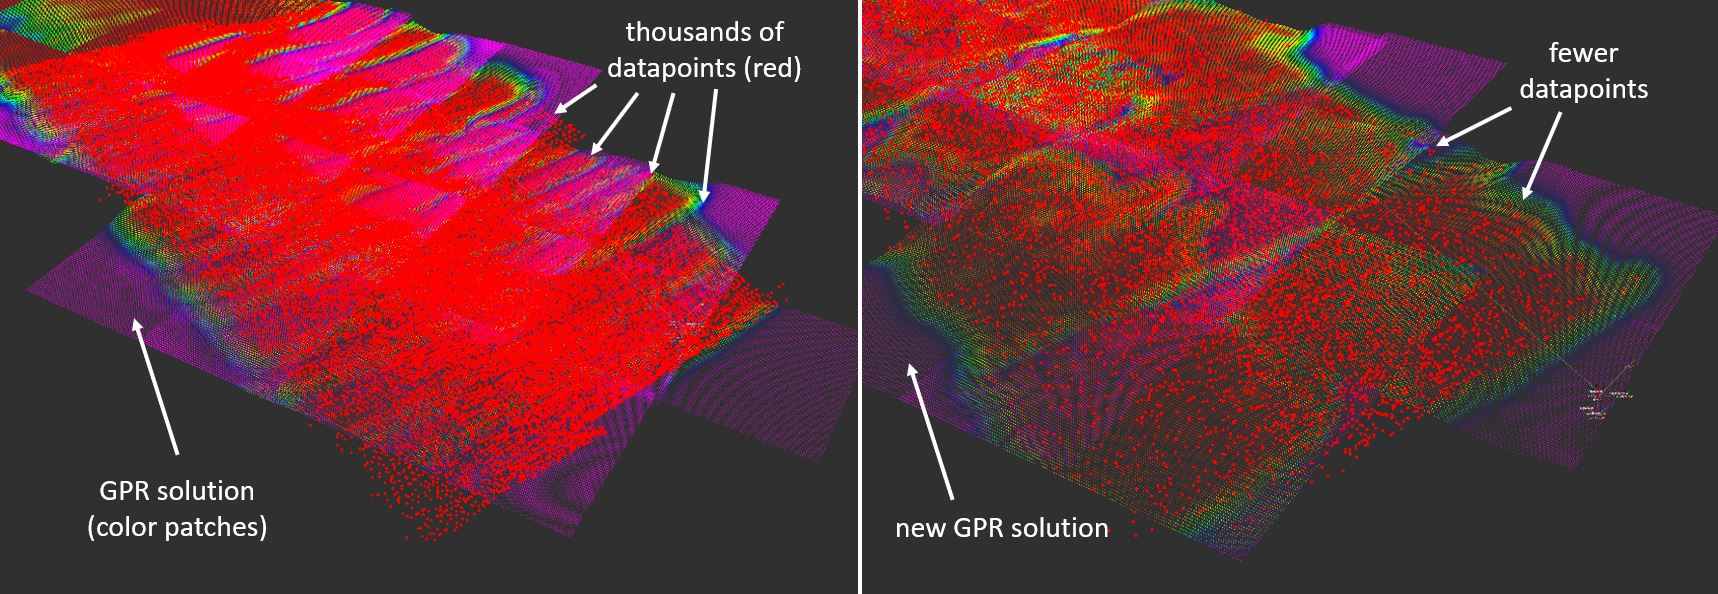
\includegraphics[width=.75\textwidth]{images/gpr_N_vs_gpr_M_pts_random_downsample_10percent.jpg}
    \end{center}
    \caption{Snapshot of ROS Rviz simulation running MP-GPR with all N points (left) and with 10\% random downsampling (right). Individual soundings (datapoints) are shown in red. GPR solution tiles are shown in color.}
    \label{fig:ROS_10percent_downsample}
\end{figure}

The dataset used in this study was collected with a WASSP sonar system in the St. Mary's River (Georgia, USA). The WASSP Multibeam Sonar retrieves a maximum of 256 points per ping at 5-20Hz depending on depth. The river is well mixed and measured sound speed profile nearly constant with depth, alleviating the need for ray tracing corrections. The mapping system and survey details are fully explained by Krasnosky, et. al \cite{KrasnoskyPOS}. 

\subsection{System Overview}\label{sec:system_overview}

The processing workflow (\ref{fig:system_block_diagram}) is setup to ingest a live sonar data stream one ping at a time. A navigation solution paired to each sonar ping accounts for dynamic effects and positions the data in the correct mapping frame. Sonar pings are passed to a 'blockulator.' The blockulator applies an outlier filter to remove erroneous soundings and downsamples the data. The filtered sonar pings are queued into tiles. GPR inference is performed on the tiles to generate predictive points with uncertainties, which are added to the bathymetry map. This is a continuous process throughout a survey \cite{Krasnosky2022}. 

\begin{figure}[!ht]
    \begin{center}
       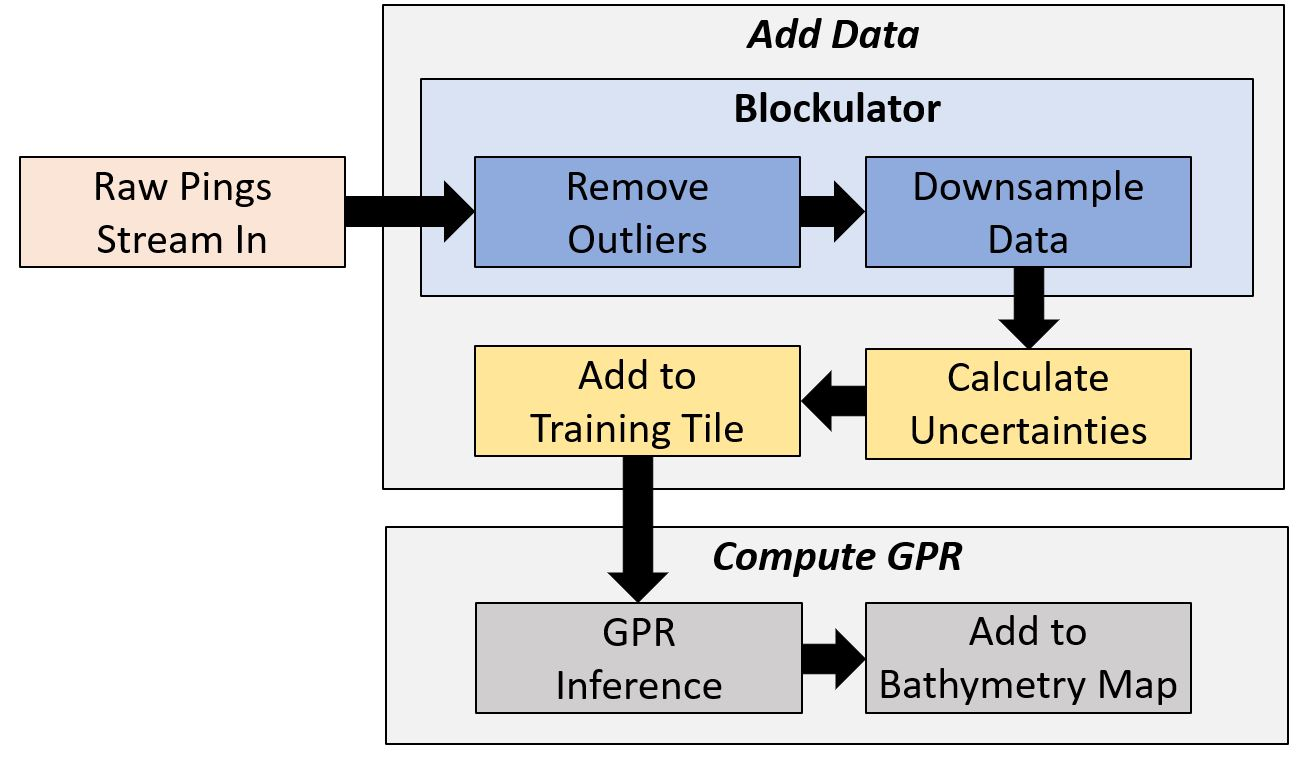
\includegraphics[width=.75\textwidth]{images/system_overview_MPGPR.jpg}
    \end{center}
    \caption{Block diagram showing MP-GPR data flow.}
    \label{fig:system_block_diagram}
\end{figure}

The downsampling methods considered are:
\begin{itemize} [noitemsep]
    \item a \textit{Uniform Random} method that selects points using a uniform random distribution,
    \item a \textit{Systematic Random} method that selects every $j$th point (decimation),
    \item a \textit{Random Hybrid} method that evenly combines systematic and uniform random selection,
    \item a \textit{Point Averaging} method that averages dense local points into a set of sparse points,
    \item a \textit{Dissimilar Neighbor} method that uses a ratio of distances to select `interesting' points,
    \item and a \textit{K-means} method that clusters points into groups based on similarity.
\end{itemize}

\subsection{Downsampling}\label{sec:downsampling}

The downsampling methods are cheap to compute and implemented as a pre-processing step as live data streams in during a multi-beam survey. Each ping of sonar data is downsampled when received ($D$ with $N$ points into $D_R$ with $M$ points) without consideration of any previously collected data. Downsampled pings are queued into blocks which are processed periodically and added to the GPR solution. The resulting time complexity is approximately $O(M^3)$.

As some downsampling methods select the most `unique' values from a set of points, outliers may be included more often than real data. The WASSP has a built-in filter to remove significantly irregular points, yet poor points may persist. Thus, an additional outlier filter was added before downsampling. A given point $p$ was considered an outlier if its depth value exceeded 2.25x the standard deviation of the neighboring points' mean (excluding $p$). Outliers were removed from the set, and the clean set was passed to the following downsampling algorithms.   

\subsubsection{Uniform Random}

Uniform random sampling is a common and fast method for downsampling. For each sonar ping, a new random seed for used to prevent bias. Uniform random sampling is used as the benchmark for evaluating the performance of other methods.

\subsubsection{Systematic Random}

Systematic random sampling ("decimation") sorts the data by a pre-determined `ordered variable' and selects every $jth$ point along that dimension. Sonar data be systematically selected using ordered indices (e.g. in MATLAB ($x_o:j:x_{end}$)). To avoid along track selection bias, the first index of each ping $x_0$ was uniform randomly selected and subsequent points were systematically selected.

\begin{figure}[!ht]
    \begin{center}
       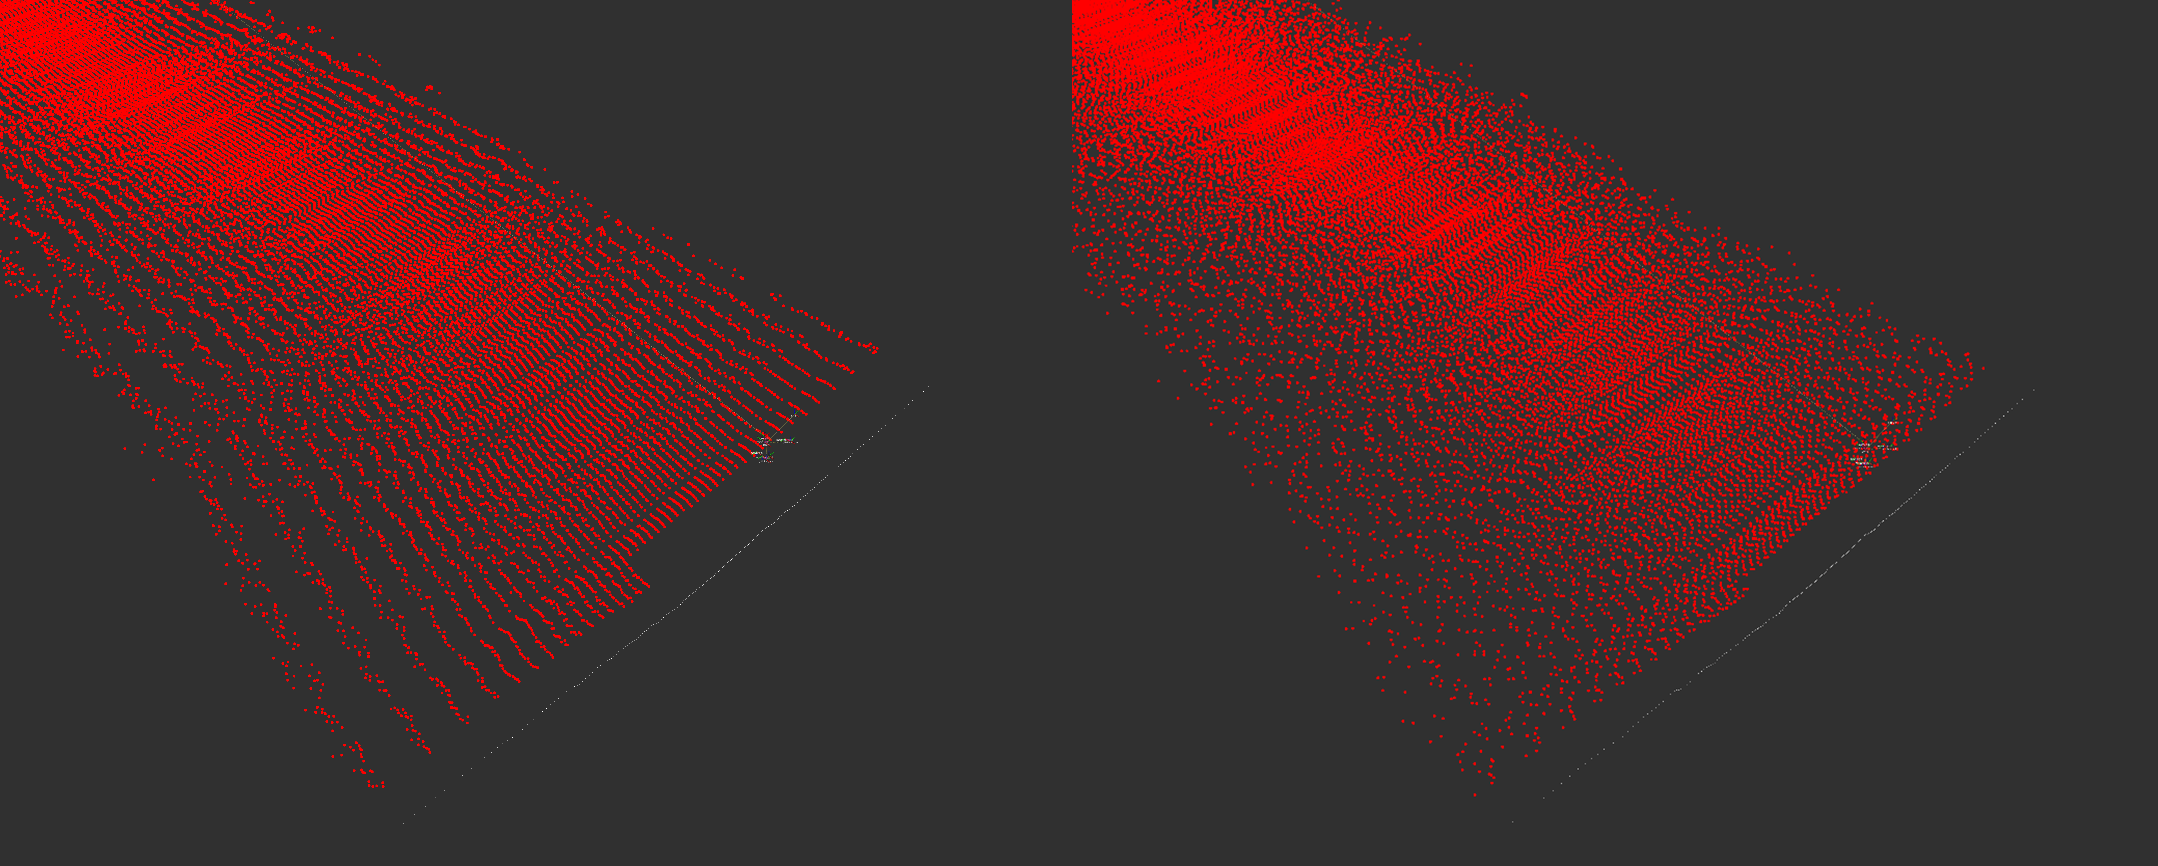
\includegraphics[width=.75\textwidth]{images/systematic_sidebyside_random_vs_norandom.png}
    \end{center}
    \caption{20\% systematic downsampling with biased (left) and unbiased (right) approaches}
    \label{fig:systematic_random_sampling_bias}
\end{figure}

\subsubsection{Hybrid Random}

The hybrid random method recognizes the value in both random and systematic sampling. Thus, half of  $D_R$ is selected spatially with systematic sampling. Then, the second half is selected from the remaining points using a uniform random distribution.

\subsubsection{Point Averaging}

Point averaging takes the average of local datapoints to create a new representative datapoint. In this manner, information from all data points influences the solution. 

%\subsubsection{Information Gain}

%The information gain algorithm \cite{Seeger2003}, $\Delta i$, uses an informative heuristic to select datapoints. There are two sets of data, a set of inclusion points $P$ (initially with one random point from $R$) and a set of raw points $R$ (initially full less one). Using a greedy selection criteria $\Delta i$, all points in $R$ are considered for inclusion into $P$. $\Delta i$ is a measure of 'information gained' by adding a point from $R$ into $P$; the $\Delta i$ value relies on a cheap approximation to the Kullback-Liebler divergence. The point in $R$ that has the highest $\Delta i$ is moved from $R$ to $P$. The process repeats itself until there are sufficient values in $P$, after which $R$ is discarded. 

\subsubsection{Dissimilar Neighbor}

The k-nearest-neighbor (KNN) algorithm is commonly used in machine learning for classification and regression. KNN uses a difference metric to determine if a new point is more similar to one group than another. The base assumption is that points with small nearest neighbor distances are more likely to be similar to their neighbors \cite{anderberg2014kmeans}. 

In the spirit of seeking `unique' points to represent the distribution of a sonar ping, similar neighbor checks the two neighboring points of $p_i$, $p_{i-1}$ and $p_{i+1}$, and calculates Euclidean distances $d_p$. Points that have the smallest distance ratio $d_r = min(d_p) / max(d_p)$ become inclusion points. A point with a ratio close to 1 is evenly-spaced with its neighbors and assumed to be uninteresting, and vice versa. A ratio is used to scale distances as the spacing of points along a ping vary. 

\subsubsection{K-means}

K-means is a popular clustering algorithm that splits a group of samples into k-clusters (subgroups) based on their similarity \cite{kmeans_inefficient}. To combat performance issues \cite{kmeans_inefficient} and keep processing time minimal, every $j$th point is selected as the initial centroids and the number of iterations are limited. The centroids of k-clusters serve as the new datapoints. 

\subsubsection{Downsampling Implementation}

Each method has one adjustable parameter: \textit{downsample percent}, $s$. A small $s$ value drastically reduces compute time and decreases solution accuracy, and vice versa. $s$ was systematically varied for each method to determine the optimal value that minimizes compute time while maximizing solution accuracy (above 98\%).

\begin{figure}[!ht]
    \begin{center}
       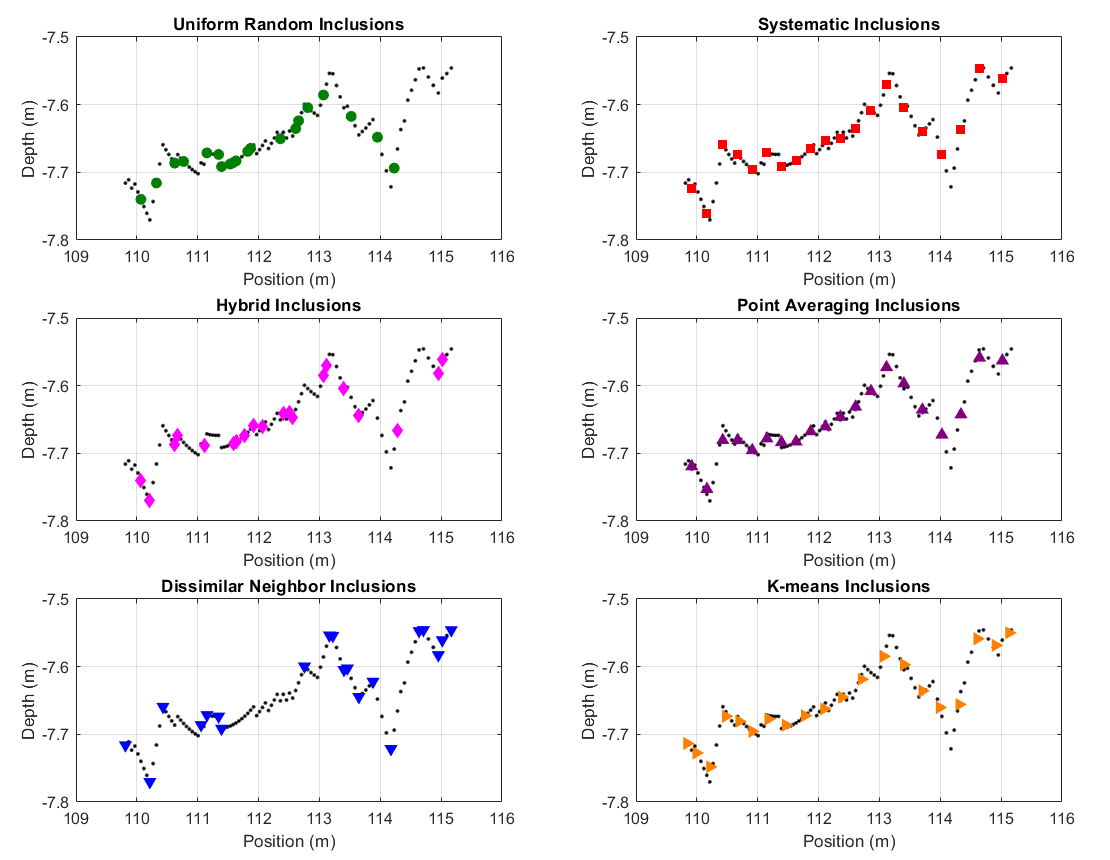
\includegraphics[width=1\textwidth]{images/eachDownsampleMethodSelectionsFig2.png}
    \end{center}
    \caption{Inclusions ($D_R$) at 20\% downsampling for each method. Data has 100 soundings of a sonar ping and each method has 20 soundings.} \label{fig:downsample_datapoints_examples}
\end{figure}

\subsection{Hyperparameter Training}\label{handling_hyperparameters}

Optimal kernel hyperparameters $\boldsymbol{\theta} = \{l,\sigma_f^2\}$ maximize the log marginal likelihood (LML) \cite{Rasmussen2006}. LML rewards model fit and punishes model complexity. It is far too computationally cumbersome to calculate LML using large datasets. Thus, the training process was performed offline before running a survey. This can be done using a small patch of bathymetry data to calculate a LML heat map over ranges of $l$ and $\sigma_f^2$ (alternatively, gradient descent can be used). The largest LML value determines the selection of $\boldsymbol{\theta}$. These parameters are inputted to MP-GPR upon starting a survey. Every variation of downsample percent $s$ for each downsample method requires retraining $\boldsymbol{\theta}$.

Note that $\boldsymbol{\theta}$ is trained on a small portion of the actual survey region. The patch should contain common features that are encountered throughout the survey. Once the hyperparameters are trained on the patch, the model applies those parameters to calculate a solution for the entire survey.

\subsection{Incorporating Uncertainty}\label{sec:uncerainty_considerations}

MP-GPR assumes each training datapoint contains the same uncertainty value $\sigma_n^2$. Uncertainty values are stored in $W$, the sensor noise matrix, such that $\boldsymbol{W} = \boldsymbol{I} \sigma_n^2$ where $\boldsymbol{I}$ is an $N \times N$ identity  matrix. Each datapoint has one associated uncertainty value that represents a $d$-dimensional Gaussian distributed error. 

Data collected by MBES are subject to multiple uncertainty sources, such as roll error, pitch error, heave error, refraction error (due to the sound speed profile), sonar system error, etc. \cite{HareMBES1995}. Importantly, each data point obtained using a sonar system has unique uncertainty values in every input dimension (northing, easting, and depth). 

For a given data point, GPR expresses $d$-dimensional uncertainties with a single value which can be visualized as a `3D uncertainty sphere' around the data point. $\sigma_n^2$ is properly expressed as an uncertainty vector $\boldsymbol{\sigma_n^2} = [\sigma_1^2, \sigma_2^2, ... \sigma_N^2]^T$ with each uncertainty value corresponding to a point in $\boldsymbol{x}$. The sensor noise matrix becomes $\boldsymbol{W} = diag(\boldsymbol{\sigma_n^2})$. Due to this formulation, capturing the dominant sources of uncertainty will include secondary error sources in other dimensions within the uncertainty sphere. Calculating $\boldsymbol{\sigma_n^2}$ must be cheap as to not subvert the computational gains from downsampling.  

capturing error in training data target values $\boldsymbol{y}$, water depth, was prioritized. A dominant source of depth error comes from the MBES's range and beam angle uncertainty. Outer beams in a sonar ping are subject to greater uncertainty than the inner beams. For a given beam angle $\phi_i$ and range $r_i$, the depth $y_i$ and uncertainty $\sigma_i^2$ for each data point can be can be calculated as,
\begin{gather*}
    y_i = r_i \cos(\phi_i) \\
    \sigma_i^2 = \sigma_{d_i}^2 = \left( \frac{\partial y_i}{\partial r_i} \sigma_r \right)^2 + \left( \frac{\partial y_i}{\partial \phi_i} \sigma_{\phi} \right)^2 \\
    \sigma_i^2 = \left( \cos(\phi_i) \sigma_r \right)^2 + \left( r_i sin(\phi_i) \sigma_{\phi} \right)^2 
\end{gather*}

The range standard deviation is sonar system dependent, and the WASSP used in these surveys reported range resolution of 0.1m ($\pm 0.05$m). Assuming a $6\sigma$ reported measurement, $\sigma_{r} = 0.1 / 6 = 0.0167$m. Beam angle resolution can be roughly estimated as total beam width divided by the number of beams. For the WASSP with a 120-degree beam width and 256 beams, $\sigma_\phi = \frac{2\pi/3}{256} = 0.0081$ radians/beam.
\begin{figure}[!ht]
    \begin{center}
       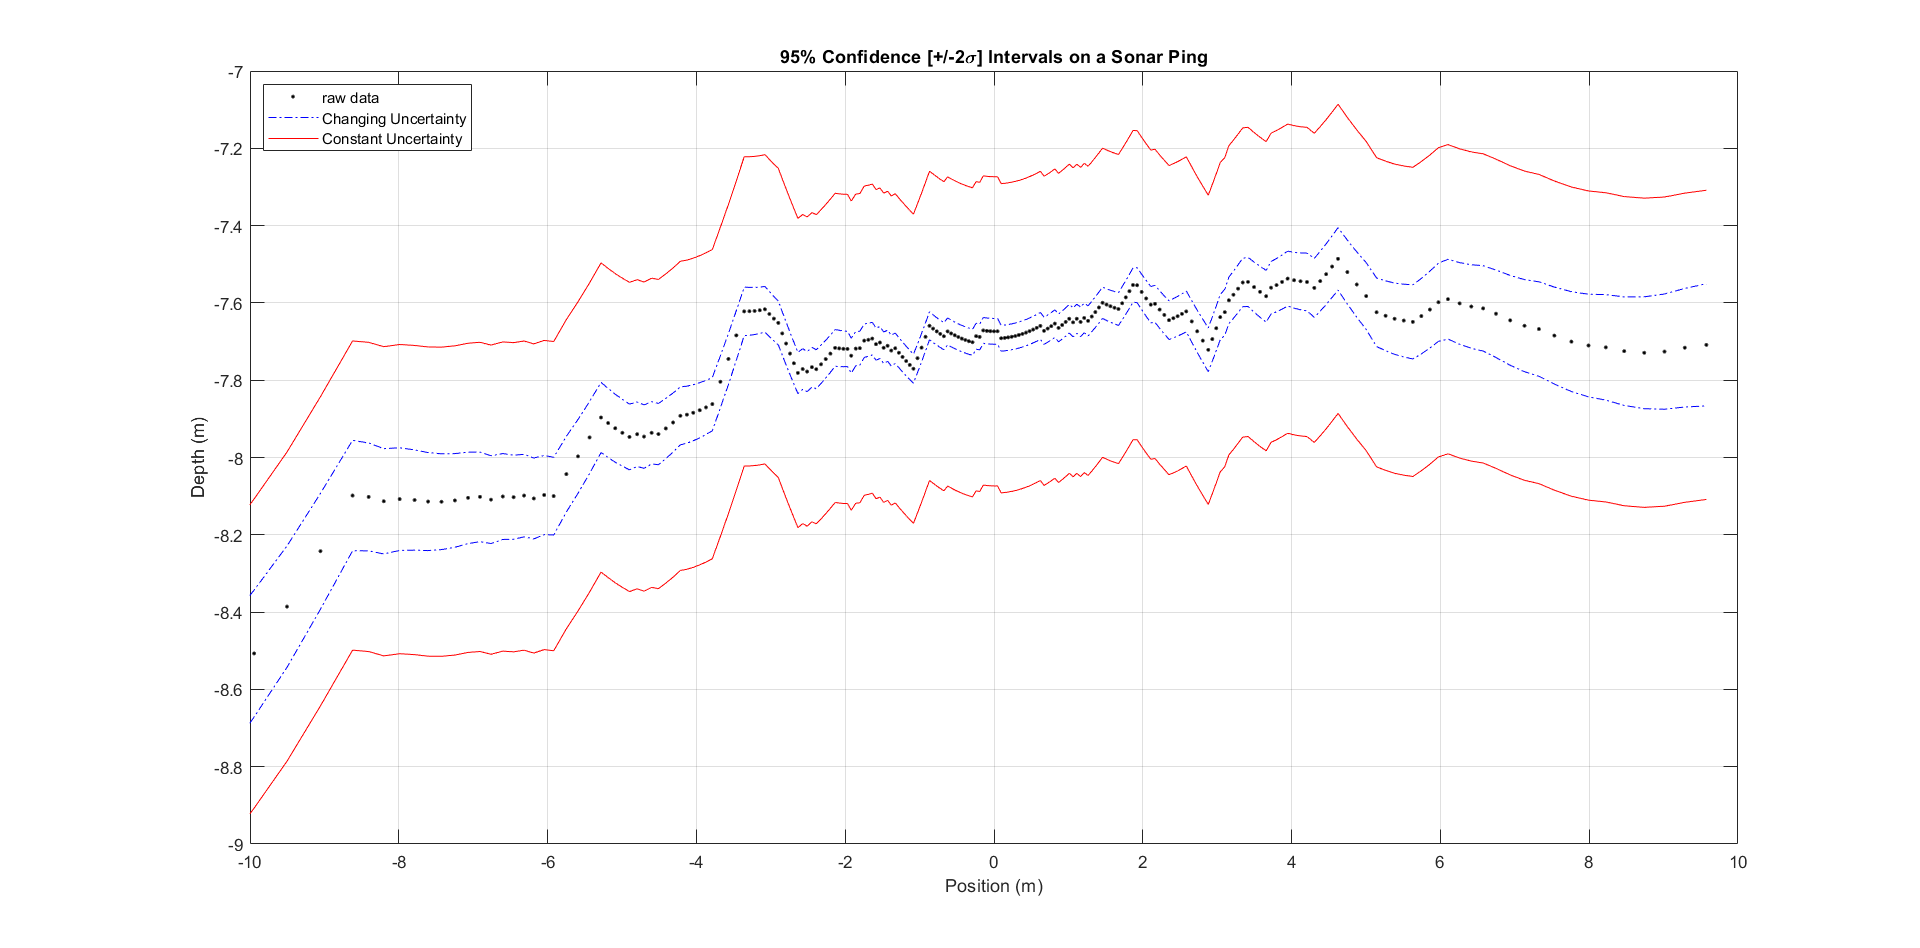
\includegraphics[width=1\textwidth]{images/ChangingvsConstantUncertaintiesPing.png}
    \end{center}
    \caption{Uncertainty values for a given sonar ping (across track) for changing uncertainties (dashed blue) and constant uncertainties (solid red).} \label{fig:uncertainty_ping}
\end{figure}
  
\section{Results}\label{sec:results}

By varying downsample percent $s$ for each downsample method, compute time and solution accuracy can be compared to the exact MP-GPR solution.

\begin{figure}[!ht]
    \begin{center}
       
\includegraphics[width=.75\textwidth]{images/blank.png}
    \end{center}
    \caption{Compute time vs. downsample percent for different approximate methods} \label{fig:computeVSdownsample}
\end{figure}

\begin{figure}[!ht]
    \begin{center}
       
\includegraphics[width=.75\textwidth]{images/blank.png}
    \end{center}
    \caption{Table showing accuracy, compute time, and downsample percent for different approximate methods} \label{fig:accuracy_time_downsample_money_chart}
\end{figure}

WHICH METHOD PERFORMED BEST?

\section{Discussion} \label{sec:discussion}

INCOMPLETE


\subsection{Future Work}

Currently, operations such as downsampling were performed on each sonar ping. Expanding the operations to run over tiles (multiple pings gathered together over time) may show improvements. This could cause along track and across track data density to be similar, improving GPR inference. This tile-by-tile approach would also enable calculation and comparison of 3D surface normals to contribute to the uncertainty analysis. CUBE \cite{calder2003automatic}, a statistical processing algorithm for multi-beam sonar, could be integrated into MP-GPR to provide uncertainty estimates at each sounding as well. 

A logical next step is preparing MP-GPR for field work. MP-GPR should be compiled on an embedded system with a GPU, such as the Nvidia Jetson Xavier, and deployed on an AUV/ASV for seafloor mapping. The maximum uncertainty points from GPR inference could be passed to an autonomous path-planning algorithm for re-mapping of low confidence areas. As any variables (not only seafloor depth) can be inputted to GPR, the algorithm is primed to map other variables such as salinity, temperature, ocean current, or other spatially distributed environmental variables.  

\section{Conclusions}\label{sec:conclusion}

INCOMPLETE
This thesis builds upon the MP-GPR algorithm by introducing multiple downsampling methods to reduce required compute time and by accounting for uncertainty values of each sonar datapoint.\cite{Rasmussen2006}



